\section{Simon's Algorithm}
Simon's algorithm was one of the first to show quantum advantage; it solves an \mathtt{NP}-hard problem in polynomial time using a quantum computer. \\\\
Given a polynomial-time computable function $f:\{0,1\}^n \to \{0,1\}^n$ it finds value $s\neq0^n$ for which $\forall x:f(x)=f(x\otimes s)$ if such $s$ exists. The function $f$ is an oracle, meaning that we don't have direct knowledge of how it computes its values.
\subsection{The algorithm}
In the algorithm we perform a quantum subroutine $n$ times. This subroutine, which quantum circuit we attach in figure \ref{fig:simon}, starts with $2n$ qubits initialized to $\ket{0}$, split into two registers with length $n$.\\
\begin{figure}[ht!]
    \centering
    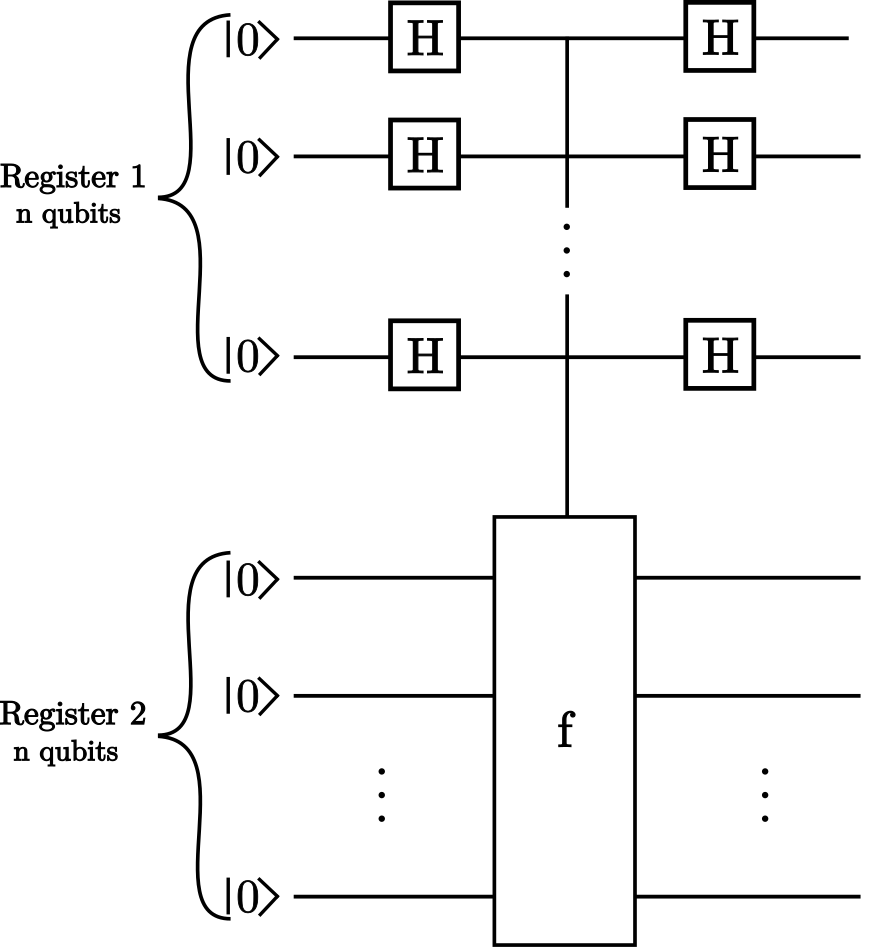
\includegraphics[width=0.65\linewidth]{30_licencjat/tex/figures/simon.png}
    \caption{Simon's algorithm subroutine circuit}
    \label{fig:simon}
\end{figure}\newpage
We first use $n$ Hadamard gates to set the first register to a uniform state, resulting in the state:
\begin{align*}
    \ket{\chi}=\frac{1}{\sqrt{2^n}}\sum_x \ket{x}\ket{0}
\end{align*}
then we apply function $f$ to the second $n$ bits giving us:
\begin{align*}
    \ket{\chi}=\frac{1}{\sqrt{2^n}}\sum_x \ket{x}\ket{f(x)}
\end{align*}
and then again apply the Hadamard gate to all qubits in the first register.
\begin{align*}
    \ket{\chi}=\frac{1}{2^n}\sum_{x,y} (-1)^{xy}\ket{y}\ket{f(x}
\end{align*}
if we change the sum to sum over all images or $f$ rather than inputs we can write as:
\begin{align*}
    \ket{\chi}=&\frac{1}{2^n}\sum_{y,f(a)}((-1)^{a\cdot y}+(-1)^{(a\oplus s)\cdot y}\ket{y}\ket{f(a)}=\\
    &=\frac{1}{2^n}\sum_{y,f(a)}(-1)^{a\cdot y}(1+(-1)^{sy})\ket{y}\ket{f(a)}
\end{align*}
if $f(x)$ was in the second register before the last gate, then in the first register there is either $a$ or $a\oplus s$ as $f(a)=f(a\oplus s)$.\\\\
Now, we notice that if two solutions ($a, a\oplus s$) exist then it must be that $s \cdot y=0$. We are only summing over values where two solutions exist thus we get:
\begin{align*}
    \ket{\chi}=\frac{1}{2^{n-1}}\sum_{y,f(a)}(-1)^{a\cdot y}\ket{y}\ket{f(a)}
\end{align*}
if we then perform a measurement on the first $n$ qubits, $y$ is selected among all values such that:
\begin{align*}
    s\cdot y = 0
\end{align*}
By itself, $y$ is not enough to compute $s$, we need to repeat this subroutine until we find $n-1$ linearly independent equations ($s\cdot y_1,\dots ,s\cdot y_n$). We only need $n-1$ rather than $n$ values, as we already assumed that $s\neq 0^n$.\\\\
Once we have $n-1$ linearly independent solutions, we can find $s$ classically in polynomial time using Gaussian elimination \cite{cormen2009}.\\\\
We still have to bound the probability that resulting equations are linearly independent. Equation $s_i$ is linearly independent if it can't be expressed as a combination of rows $\{1,s_{i-1}\}$, therefore the probability of all equations being linearly independent is  
\begin{align*}
    \prod_{k=0}^{n-1} \left(1-\frac{2^k}{2^n}\right)=\prod_{k=0}^{n-1} \left(1-\frac{1}{2^{n-k}}\right)=\prod_{k=1}^{n-1} \left(1-\frac{1}{2^{k}}\right) \geq 0.288
\end{align*}
We can always repeat this process to increase the probability of success.\subsection{Complexity and impact}
The bound is not dependent on $n$, therefore only a constant number of trials is needed to increase the probability of success above any threshold, therefore the algorithm is in $\mathtt{BQP}$.\\\\
It will with high probability perform $n-1$ subroutines each requiring $2n$ Hadamard operations and a call to function $f$, thus the complexity is $O(n^2 \text{poly(n)})$.\\\\
Simon's algorithm was the first algorithm to separate $\mathtt{BPP}$  from $\mathtt{BQP}$, it showed an exponential advantage as the best known classical algorithm is $O(2^{n/2}\text{poly(n}))$, which is why it inspired others to seek more complex algorithms, solving more practical problems such as Shor's algorithm for factorisation.
